\documentclass[thesis.tex]{subfiles}
\begin{document}
In the previous chapter, the classical (or standard) residual error estimator is introduced as the driver for the
adaptive finite element method (AFEM). This results in an optimal algorithm, i.e.~the adaptive meshes
generated by this method provide the highest possible convergence rate. Unfortunately, this asymptotic result
is a bit inconvenient for practical purposes due to the unknown constants. In practice,
one would like to know \emph{when} to stop iterating, i.e.~when the approximation error is small enough --- say
below some threshold. 

Another problem of the classical residual error estimator is that it is not polynomial-degree-robust: 
the constants depend on $p$, the degree of the finite element solutions. This becomes an issue
when considering \emph{hp}-AFEM, a version of AFEM where the polynomial degree can also vary
per element. For \emph{hp}-AFEM, one would like an estimator with constants independent of the polynomial degree
used on each of the elements.

Conveniently, there are error estimators that suffer less from these constants problems. Recently, quite
some research interest has been shown for such constant-free estimators. One of these estimators is the
\emph{equilibrated residual error estimator}, also called the \emph{equilibrated flux estimator} or the \emph{Braess-Sch\"oberl estimator}
\cite{braessequil, braessequilrobust,ernequil}.
In this chapter, we will introduce this estimator --- which we will refer to as the equilibrated flux estimator --- and prove some
of its properties. 

For simplicity, we restrict ourself to the Poisson problem \eqref{eq:poisson} on a two-dimensional polygonal domain $\O \subset \R^2$,
with a right hand side $f \in L^2(\O)$. For some conforming triangulation~$\T$ of the domain,  we consider $\VV := \VV(\T)$ --- the (Lagrange) finite
element space of degree $p\geq 1$. We assume each triangulation to be uniformly shape regular, i.e.~$\sup_{K \in \T} h_K/p_K \leq \kappa$ for
some shape regularity constant $\kappa$.
The Galerkin approximation (discrete solution) is denoted by $U \in \VV(\T)$.
\section{Prager and Synge}
The so-called equilibrated flux estimators are based on the fundamental theorem of Prager and Synge \cite{prager},
for which, we need the space $H(\div; \Omega)$ as defined in \ref{def:hdiv}. Vector-valued functions will be underlined.
%to emphasize their difference to scalar-valued functions.
\begin{thm}[Prager and Synge]
  \label{thm:prager}
  Let $u \in H_0^1(\O)$ be the exact solution of the Poisson problem with a right hand side $f \in L^2(\O)$. 
  For a flux $\v{\sigma} \in H(\div; \O)$ satisfying the equilibrium condition $\div \v{\sigma} + f = 0$ in $L^2$-sense, there holds
\[
  \norm{\nabla u - \nabla v}^2_{\O} + \norm{\nabla u - \v{\sigma}}^2_{\O} = \norm{\nabla v - \v{\sigma}}^2_{\O} \quad \forall v \in H_0^1(\O).
\]
\end{thm}
\begin{proof}
  Application of the divergence theorem \eqref{thm:divergence} yields
  \begin{align*}
    &\int_\O  \left(\nabla u - \v{\sigma}\right) \cdot \nabla \left( u -  v\right)  \, \dif x \\ 
    =  - &\int_\O \left(u - v\right) \,  \div \left (\nabla u - \v{\sigma}\right) \dif x + \int_{\partial \O} (u - v) \left( \nabla u \cdot n - \v{\sigma} \cdot n\right) \dif s  = 0,
  \end{align*}
  since from the assumptions  $\Delta u = -f = \div \v{\sigma}$ in $\O$, and $u - v = 0$ on $\partial \O$.
  From this orthogonality relation and Pythagoras' identity we may conclude that
  \[
    \norm{\nabla(u-v)}^2_{\O} + \norm{\nabla u - \v{\sigma}}^2_{\O} = \norm{ -\nabla (u-v) + \nabla u - \v{\sigma}}^2_{\O},
  \]
  which equals the asserted.
\end{proof}
For a flux $\vsig$ satisfying the equilibrium condition, we obtain an 
\emph{reliable} constant-free estimator by replacing $v$ with the discrete solution $U$ in the previous theorem:
\begin{equation}
  \label{eq:synest}
  \enorm{u - U}_{\O}^2 =  \norm{\nabla u - \nabla U }^2_{\O} \leq \norm{\nabla U - \vsig}^2_{\O}.
\end{equation}

The question now arises how to construct $\vsig$. In general one would like an estimator to be proportional to the error.
For this, we need the estimator to also be \emph{efficient}: it should provide a lower bound for $\enorm{u -U}_{\O}$, up to
a constant and possibly an oscillation term. The following construction will provide such efficiency.

From now until \S\ref{sec:oscillation}, we suppose that $f$ is a piecewise polynomial of degree at most $p-1$ on $\T$, i.e.
\[
  f\in \P_{p-1}^{-1}(\T) := \set{ f \in L^2(\O): f|_K \in \P_{p-1}(K) \quad \forall K \in \T},
\]
and consider the  $p$-th order \emph{Raviart-Thomas} \cite{raviart1977mixed}  space $\RT_p(\T)$ defined by:
\begin{align*} 
  \RT_p(K)    &:= \left[ \P_p(K)\right]^2 + \P_p(K)\v{x}, \\
  \RT_p^{-1}(\T) &= \set{ \v{\sigma} \in \left[L^2(\O)\right]^2 : \v{\sigma}|_K \in \RT_p(K) \quad \forall K \in \T},\\
  \RT_p(\T) &:= H(\div; \O) \cap \RT_p^{-1}(\T).
\end{align*}
Evidently fluxes $\v{\sigma} \in \RT_p(K)$ satisfy $\div \v{\sigma} \in \P_p^{-1}(\T)$; the divergence mapping
is even surjective \cite[Prop~2.3.3]{brezzimixed}, and thus $\RT_p(K)$ contains equilibrated fluxes.
 From~\eqref{eq:synest} we then see that 
the sharpest estimator in the Raviart-Thomas space is found by minimizing $\norm{\nabla U - \sigma}$ over all 
fluxes $\v{\sigma} \in \RT_p(\T)$ that are in equilibrium. However,
this global minimization procedure --- equivalent to the mixed finite element solution \cite{braess2007finite} --- 
is too expensive for computation of an error estimate.

To overcome this problem, Braess and Sch\"oberl \cite{braessequil} propose minimizing local problems instead, a procedure
called \emph{equilibration}.

\section{Equilibration} 
Instead of directly constructing the flux $\v{\sigma}$, the difference $\v{\sigma}^\triangle := \nabla U -  \v{\sigma}$ is considered.
We assume that $f$ belongs to the broken polynomial space $\P_{p-1}^{-1}(\T)$ to avoid the effect of
data oscillation.  The flux $\v{\sigma}$ will be constructed in $\RT_p(\T)$; the correction~$\vsig^\triangle$ must 
therefore belong to the broken Raviart-Thomas space $\RT_p^{-1}(\T)$.

Following \cite{ernequil}, we use $\V, \E$ to denote  the set of vertices and edges in the triangulation~$\T$. 
Superscripts  $^{int}$ or $^{bdr}$ are added to indicate restrictions of $\V, \E$ to the interior or the boundary.
For each vertex $a \in \V$, we write $\psi_a$ for the hat function at vertex $a$, 
i.e.~the unique function in the linear finite element space
that takes value $1$ at $a$ and vanishes at the other vertices.
These hat functions form a partition of unity: $\sum_{a \in \V} \psi_a \equiv \1$.
The local problems are solved on patches $\omega_a$, given by the star at a vertex $a \in \V$, also being the support of
the hat function $\psi_a$ --- see Figure~\ref{fig:patches} for an illustration. We denote $\gamma_a$ for the union of interior edges touching $a$. 
So for a vertex $a \in \V$ we have
\[
  \omega_a       := \omega\left(\T, a\right) = \bigcup \{ K \in \T : a \in \partial K\},
  \quad \gamma_a := \gamma\left(\T, a\right) = \bigcup \{ e \in \E^{int} : a \in e\}.
\]
Often we are interested in the set of elements $K \in \T$ that make up $\w_a$. We abuse the notation and intuitively write $K \subset \w_a$
under sums as shorthand for $\set{K \in \T : a \in \partial K}$; similarly we write $e \subset \gamma_a$ to mean $\{e \in \E^{int} : a\in e\}$.
 
\begin{figure}
  \centering
  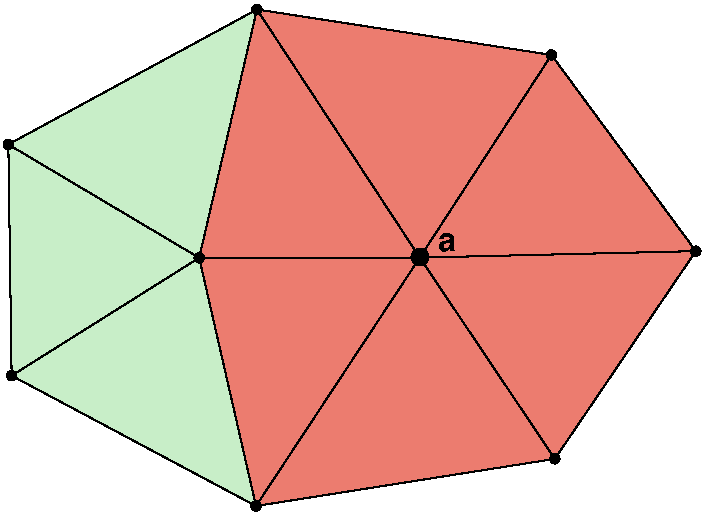
\includegraphics[width=.45\linewidth]{mesh/ex_intpatch.pdf}
  \quad
  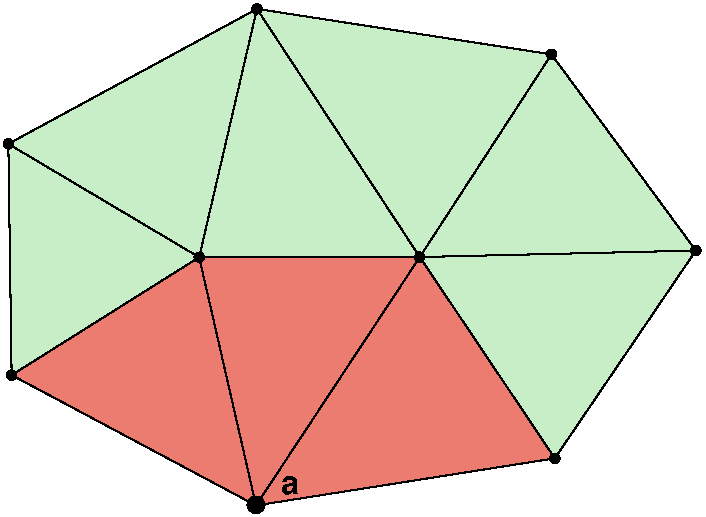
\includegraphics[width=.45\linewidth]{mesh/ex_bdpatch.pdf}
  \caption{Two different type of patches highlighted. The left image displays a patch~$\w_a$  associated to an interior vertex $a$.
  The right image displays a typical patch associated to a boundary vertex.}
  \label{fig:patches}
\end{figure}
  
For each patch $\w_a$, we solve a local problem resulting in a local flux $\vsiga$. 
The total difference flux $\v{\sigma}^\triangle$ is then taken as the sum of local fluxes over these patches, 
\[
  \v{\sigma}^\triangle := \sum_{a \in \V} \vsiga.
\] 
As proposed  in \cite{braessequilrobust}, local fluxes are found by decomposing the residual using the partition of unity. 
Write $r \in H_0^1(\O)'$ for the usual residual defined in \S\ref{sec:afem}, i.e.~for $v\in H_0^1(\O)$ 
\[
  \ip{r,v} := a(u - U, v) = \ip{\nabla \left(u - U\right), \nabla v}_\O = \ip{f,v}_\O - \ip{\nabla U,\nabla v}_\O.
\]
For every vertex $a \in \V$, the local residual at $a$ is defined as
\[
  \ip{r_a,v} := \ip{r,\psi_a v} = a(u - U, \psi_a v)_{\w_a}.
\]
The local flux $\vsiga$ is taken from the broken Raviart-Thomas space $\RT_{p}^{-1}(\omega_a)$ such that
\begin{equation}
  \label{eq:defsigma}
  \ip{r_a, v} = - \ip{\v{\sigma_a}, \nabla v}_{\w_a} \quad \forall v \in H^1(\w_a) \cap H_0^1(\O).
\end{equation}
Existence of such a flux $\vsiga$ will be shown at the end of this section.
The residual can be expressed in triangle and edge related terms by applying the divergence theorem, cf.~\eqref{eq:residualdecomp}.
This leads to the decomposition
\begin{equation}
  \label{eq:locdecomp}
  \ip{r_a,v} = \ip{f, \psi_a v}_{\w_a} - \ip{\nabla U, \nabla (\psi_av)}_{\w_a} = \sum_{ K\subset \w_a} \langle{r^T_a, v}\rangle_K + \sum_{ e \subset \gamma_a} \ip{r^e_a, v}_e,
\end{equation}
with $L^2$-inner products over elements $K$ and (lower dimensional) edges $e$, and
\[
  r^T_a := \psi_a \left[ f + \Delta U \right], \quad r^e_a := \psi_a \llbracket \nabla U \rrbracket.
\]
Similarly rewriting $\ip{\v{\sigma_a}, \nabla v}_{\w_a}$ in triangle and edge related terms yields
\[
  -\ip{\v{\sigma_a}, \nabla v}_{\w_a} = \sum_{K \subset \w_a} \ip{\div \v{\sigma_a}, v}_K + \sum_{ e\subset \gamma_a} \ip{\llbracket \v{\sigma_a}\rrbracket, v} + \ip{\vsiga\cdot n, v}_{\partial \w_a \setminus \partial \O}.
\]
After expanding both sides, we see that \eqref{eq:defsigma} holds if and only if
\begin{equation}
  \label{eq:sigmacons}
  \begin{alignedat}{3}
    \div \v{\sigma_a} &= \psi_a \left [f + \Delta U\right] && \quad\text{in }  K\subset \w_a ,\\
    \llbracket \v{\sigma_a} \rrbracket &= \psi_a \llbracket \nabla U \rrbracket && \quad \text{on } e \subset \gamma_a,\\
    \v{\sigma_a} \cdot n &= 0 &&\quad \text{on } \partial \w_a \setminus \partial \O.
  \end{alignedat}
\end{equation}
To prove that system \eqref{eq:sigmacons} has a solution we make the following observation.
For an interior vertex $a \in \V^{int}$, the hat function $\psi_a$ belongs to the finite element space~$\VV(\T)$. 
Using that $U$ is the Galerkin approximation therefore gives us $\ip{r_a,\1} = \ip{f, \psi_a}_\O - \ip{\nabla U, \nabla \psi_a}_{\O} = 0$.
That is, the local residual vanishes on constant functions.
\begin{thm}
  \label{thm:sigmasolvable}
  There exists a flux $\vsiga \in \RT_{p}^{-1}(\w_a)$ that solves the above system \eqref{eq:sigmacons}.
\end{thm}
\begin{proof}
  We use a (well known) result for Raviart-Thomas elements proved in Lemma~\ref{lem:rtexists}, namely, 
  for an element $K$ there exists a function $\vtau \in \RT_p(K)$ such that
  \[
    \div \vtau = P_K \, \in \P_p(K), \quad \vtau \cdot n = P_e \in \,\P_p(e) \quad \forall e \subset \partial K,
  \]
  if the polynomials satisfy the compatibility constraint $\int_K P_K = \int_{\partial K} P_e$.
  Notice that the polynomials in \eqref{eq:sigmacons} are of degree $p$, and are thus eligible in this theorem.

  Fix an interior vertex $a \in \V^{int}$. In this case, $\w_a$ is of the shape depicted in Figure~\ref{fig:patches}. Let $\set{K_1,\dots,K_n}$ be a numbering
  of the $n$ distinct elements such that $K_i$ and $K_{i+1}$ share an edge, 
  i.e.~$K_i \cap K_{i+1} =e_i \in \gamma_a$ for $1 \leq i \leq n-1$. The first and last element also share an edge $K_1 \cap K_n = e_n$,
  because $a$ is an interior vertex. The edges of $K_i$ are thus given by $e_i, e_{i-1}$ and a (patch) boundary edge $\tilde e_i$. 
  For $K_1$, we pick a $\vsign{1}\in \RT_p(K_1)$ that solves 
  \begin{equation}
    \label{eq:first}
  \begin{alignedat}{3}
    \div \vsign{1} &= \psi_a \left [f + \Delta U\right] && \quad\text{in }  K_1\subset \w_a ,\\
    \vsign{1} \cdot n  &=-\psi_a \llbracket \nabla U \rrbracket && \quad \text{on } e_n \subset \gamma_a,\\
    \vsign{1} \cdot n  &= 0 && \quad \text{on } \tilde e_1 \subset \partial \w_a,\\
    \vsign{1} \cdot n  &= p_1 && \quad \text{on } e_{1} \subset \gamma_a,
  \end{alignedat}
\end{equation}
  with $p_1$ a polynomial chosen such that the compatibility condition holds, i.e.
  \[
    \int_{K_1} \psi_a \left[ f + \Delta U\right] = \int_{e_n} - \psi_a \llbracket \nabla U \rrbracket + \int_{e_1} p_1.
  \]  
  Existence of~$\vsign{1}$
  then follows from Lemma~\ref{lem:rtexists}. Similarly, we solve $\vsign{2} \in \RT_p(K_2)$ from
  \begin{alignat*}{3}
    \div \vsign{2} &= \psi_a \left [f + \Delta U\right] && \quad\text{in }  K_2\subset \w_a ,\\
     \vsign{2} \cdot n  &= -\psi_a \llbracket \nabla U \rrbracket - p_1 && \quad \text{on } e_1 \subset \gamma_a,\\
    \vsign{2} \cdot n  &= 0 && \quad \text{on } \tilde e_2 \subset \partial \w_a,\\
    \vsign{2} \cdot n  &= p_2 && \quad \text{on } e_{2} \subset \gamma_a,
  \end{alignat*}
  for some polynomial $p_2$ that ensures the compatibility condition. Per construction the trace jump of $\vsign{1}$ and $\vsign{2}$ over
  $e_1$ equals the required $\psi_a \llbracket \nabla U \rrbracket$.
  
  We can repeat this process until we arrive at $K_n$. At this point we are no longer
  free to pick the `next'  edge polynomial $p_n$, because this is already determined by the first element in \eqref{eq:first}.
  To complete the system \eqref{eq:sigmacons} we would like to solve $\vsign{n} \in \RT_p(K_n)$~
  from
  \begin{equation}
    \label{eq:sigman}
  \begin{alignedat}{3}
    \div \vsign{n} &= \psi_a \left [f + \Delta U\right] && \quad\text{in }  K_n\subset \w_a ,\\
    \vsign{n} \cdot n  &= -\psi_a \llbracket \nabla U \rrbracket - p_{n-1} && \quad \text{on } e_{n-1} \subset \gamma_a,\\
    \vsign{n} \cdot n  &= 0 && \quad \text{on } \tilde e_n \subset \partial \w_a,\\
    \vsign{n} \cdot n  &= 0 && \quad \text{on } e_{n} \subset \gamma_a.
  \end{alignedat}
\end{equation} 
  We will show that the compatibility condition is satisfied.
  From orthogonality on constant functions we deduce
  \[
    \ip{r_a, \1} = 0 \implies \sum_{i = 1}^n \int_{K_i} \psi_a \left[f+\Delta U\right] + \sum_{i = 1}^n \int_{e_i} \psi_a \llbracket \nabla U \rrbracket = 0.
  \]
  Combining this with the compatibility conditions of $\vsign{i}$ for $1 \leq i \leq n-1$ shows
  \begin{align*}
    \int_{K_n} \psi_a  \left[ f + \Delta U \right] &=- \sum_{i = 1}^{n-1} \int_{K_i} \psi_a \left[ f + \Delta U \right] - \sum_{i=1}^n \int_{e_i} \psi_a \llbracket \nabla U \rrbracket \\
    &=   - \int_{e_1} p_1 -  \sum_{i = 2}^{n-1} \int_{K_i} \psi_a \left[ f + \Delta U \right] - \sum_{i=1}^{n-1} \int_{e_i} \psi_a \llbracket \nabla U \rrbracket \\
    &= \dots =- \int_{e_{n-1}} \psi_a \llbracket \nabla U \rrbracket - \int_{e_{n-1}} p_{n-1}.
  \end{align*}
  We see that the compatibility also holds for this last system \eqref{eq:sigman}, thereby proving existence of $\vsign{n}$.
  Defining $\vsiga|_{K_i} := \vsign{i}$ for $1 \leq i \leq n$ then provides us with a flux $\vsiga \in \RT_{p,0}^{-1}(\w_a)$ that satisfies \eqref{eq:sigmacons}.

  The process is similar for a boundary vertex $a \in \V^{bdr}$.  We can again find a numbering $\set{K_1, \dots, K_n}$
  of the elements inside the patch $\w_a$ such that $K_i \cap K_{i+1} = e_i$. This time the
  elements $K_1$ and $K_n$ do not share a boundary, since $a$ is a boundary vertex (cf.~Figure~\ref{fig:patches}). 
  The system \eqref{eq:sigmacons} does not prescribe conditions on edges of the domain boundary.
  We can therefore simply apply the method described above without having a conflict at the last element $K_n$.
  This process results in a $\vsiga$ that solves the system \eqref{eq:sigmacons}.

  \end{proof}
  From this proof it is clear that we can restrict ourselves to finding local flux $\vsiga$ in the subspace $\RT_{p,0}^{-1}(\w_a)$ defined by
  \begin{equation}
    \label{def:rtp0}
    \RT_{p,0}^{-1}(\w_a) := 
   \left[\begin{aligned}
      &\set{ \v{\sigma} \in \RT_p^{-1}(\w_a) : \v{\sigma} \cdot n = 0 \quad \text{on } \partial \w_a} & a \in \V^{int}, \\
      &\set{ \v{\sigma} \in \RT_p^{-1}(\w_a) : \v{\sigma} \cdot n = 0 \quad \text{on } \partial \w_a \setminus \partial \O} & a \in \V^{bdr}. 
  \end{aligned}
\right.
\end{equation}
  Since there is no unique solution that solves the system \eqref{eq:sigmacons}, a \emph{minimal} $L_2$-norm solution is chosen. In summary,
  the locally equilibrated flux $\v{\sigma_a}$ is given by
  \[
    \v{\sigma_a} \in \RT_{p,0}^{-1}(\w_a) \quad \text{ s.t. $\v{\sigma_a}$ satisfies \eqref{eq:defsigma} and } \uanorm{\v{\sigma_a}}_{\w_a} = \min_{\v{\sigma} \in \RT_{p,0}^{-1}(\w_a) : \v{\sigma} \text{ satisfies \eqref{eq:defsigma}}} \norm{\v{\sigma}}_{\w_a}.
  \]
  These locally equilibrated fluxes are lifted to the entire space by taking $\vsig^\triangle = \sum_{a \in \V} \vsiga$. 
  Finally set $\v{\sigma} = \nabla U - \vsig^\triangle$, then for $v \in H_0^1(\O)$ we have
\begin{align*}
  \ip{\vsig, \nabla v}_{\O} &= \ip{\nabla U, \nabla v}_{\O} - \sum_{a \in \V} \ip{\vsiga, \nabla v}_{\w_a} \\
     &= \ip{\nabla U, \nabla v}_{\O} + \sum_{a \in \V} \ip{r_a, v} \\
  &= \ip{\nabla U, \nabla v}_{\O} + \ip{r,v} = \ip{f,v}_{\O}.
\end{align*}
Since this holds for all $v \in H_0^1(\O)$, we know that $\vsig$ has a weak divergence that is given by $\div \vsig =  -f$. 
Invoking Prager and Synge then gives the desired upper bound.
\begin{thm}
  \label{thm:reliablsyn}
  The above described process provides a reliable estimator, i.e.
  \[
  \enorm{u - U}_{\O} \leq \norm{\nabla U - \v{\sigma}}_{\O} = \uanorm{\vsig^\triangle}_\O = \norm{\sum_{a \in \V} \vsiga}_\O.
\]
\end{thm}
\section{Efficiency}
\label{sec:efficiency}
The next (more involved) step is showing efficiency of the equilibrated flux estimator.
We will derive patch-wise efficiency results, because of the localized nature of the estimator.
These results will be proven using the relation between $\v{\sigma_a}$ and the local residual $r_a$.
Recall that for $a \in \V^{int}$, the functional $r_a$ vanishes on constant functions, and therefore we may interpret $r_a$
as a functional on the mean zero space. Again in the notation of~\cite{ernequil}, we define for~$a\in\V$,
\[
  H^1_\star(\omega_a) := \left[\begin{aligned}
      &\set{v \in H^1(\omega_a):  \ip{v,\1}_{\omega_a} =:v_{\omega_a}  = 0} &\quad a \in \V^{int},\\
    &\set{v \in H^1(\omega_a): v = 0 \text{ on }\partial \omega_a \cap \partial \O} &\quad a \in \V^{bdr}.
  \end{aligned}
\right.
\]
We equip this space with the norm $\norm{\nabla \cdot }_{\omega_a}$, which is a norm since 
\[
  \norm{\nabla v}_{\omega_a} = 0 \implies v = C_{st}, \quad v \in H_\star^1(\omega_a) \implies C_{st} = 0.
\]
Even stronger,
this norm is equivalent to the $H^1$-norm by Poincar\'e-Friedrichs inequality (cf.~\S\ref{sec:poincfried}).
With these definitions we are able to proof local efficiency in terms of $r_a$.
To avoid unnecessary confusion, we  will write $a \lesssim b$ if there holds $a \leq C b$ for some constant~$C$.
Similarly, we write $a \gtrsim b$ if we have $b \lesssim a$, and $a \eqsim b$ if both inequalities hold.
\begin{lem}
  \label{lem:loceff}
  For every vertex $a \in \V$, we have the following local efficiency on $\omega_a$,
  \[
    \norm{r_a}_{H_\star^1(\omega_a)'} \lesssim \enorm{ u - U}_{\omega_a},
  \]
  for a constant only dependent on the shape regularity of the triangulation --- and thus independent of the polynomial-degree $p$.
\end{lem}
\begin{proof}
  By definition and the Cauchy-Schwarz inequality we find
  \begin{align*}
    \norm{r_a}_{H_\star^1(\omega_a)'} &= \sup_{\{v \in H_\star^1(\omega_a) : \norm{\nabla v}_{\w_a} = 1\}} \abs{\ip{r_a, v}}\\
    &= \sup_{\{v \in H_\star^1(\omega_a) : \norm{\nabla v}_{\w_a} = 1\}} \abs{\ip{\nabla \left(u - U\right), \nabla \left(\psi_a v\right)}_\O} \\
    &\leq \norm{\nabla u - \nabla U}_{\omega_a} \sup_{\{v \in H_\star^1(\omega_a): \|\nabla v\|_{\w_a}=1\}} \norm{ \nabla \left (\psi_a v \right)}_{\omega_a}.
  \end{align*}
  In order to get rid of the $\psi_a$ term we first apply the product rule,
  \begin{align*}
    \norm{\nabla\left(\psi_a v\right)}_{\omega_a} &= \norm{v \nabla \psi_a + \psi_a \nabla v}_{\omega_a}\\
    &\leq \norm{v \nabla \psi_a}_{\omega_a} + \norm{\psi_a \nabla v}_{\omega_a} \\
    &\leq \norm{v}_{\omega_a} \norm{\nabla \psi_a}_{\infty, \omega_a} + \norm{\psi_a}_{\infty, \omega_a} \norm{\nabla v}_{\omega_a}.
  \end{align*}
 For the $\psi_a$ terms we note that 
  $\norm{\psi_a}_{\infty, \omega_a} = 1$, whereas $\nabla \psi_a$ is constant and bounded on each triangle by
  $\rho_{K}$, and thus $\norm{\nabla \psi_a}_{\infty, \omega_a} \leq C h^{-1}_{\w_a}$ for some constant only depending on the 
  shape regularity $\kappa$. 
  The $\norm{v}_{\omega_a}$-term can be estimated using Poincar\'e-Friedrich inequalities (cf \S\ref{sec:poincfried}):
  \[
    \norm{v}_{\omega_a} = \begin{cases}
      \norm{v - v_{\omega_a}} \leq C_{P,\omega_a} h_{\omega_a}\norm{\nabla v}_{\omega_a} & a \in \V^{int}, \\
      \norm{v} \leq C_{F,\omega_a} h_{\omega_a}\norm{\nabla v}_{\omega_a} & a \in V^{bdr},
    \end{cases}
  \]
  with the constants depending only on the shape regularity $\kappa$ of the triangulation.
  Combining these inequalities and using that $\norm{\nabla v}_{\w_a} = 1$, we arrive at the asserted.
\end{proof}

This efficiency bound can be related to the local flux $\vsiga$.
Recall that $\vsiga\in \RT_{p,0}(\w_a)$ was found to be the minimal norm function satisfying \eqref{eq:defsigma}.
 The fact that this flux is of minimum norm enabled Braess et al.~\cite{braessequilrobust} to prove the following powerful theorem.
\begin{thm}
  \label{thm:locresequiv}
  For $a \in \V$, let $\v{\sigma_a}$ be found as described above. The following efficiency bound holds for a constant depending on 
  the shape regularity, but is independent of the polynomial-degree $p$ used in the finite element space $\VV$:
  \[
    \uanorm{\v{\sigma_a}}_{\omega_a} \lesssim \norm{r_a}_{H_\star^1(\w_a)'},
  \]
  %We have an efficiency bound that holds for a constant independent of the polynomial-degree $p$ used in the finite element space $\VV$:
  %We have the bound $\norm{r_a}_{H_\star^1(\omega_a)'} \leq \uanorm{\v{\sigma_a}}_{\omega_a}$. But more importantly,
  %a reverse bound also holds for a constant {not} depending on the polynomial-degree $p$ used in the finite element space $\VV$:
\end{thm}
\begin{proof}
The proof of this theorem is very involved. A constructive proof is given in \cite[Theorem~7]{braessequilrobust}.
The theorem formulation given in \cite{braessequilrobust} is only applicable to interior vertices $a \in \V^{int}$.
By the nature of the proof, however, this result easily extends to boundary vertices $a \in \V^{bdr}$ as well (cf.~Theorem~\ref{thm:sigmasolvable}). 
\end{proof}
\begin{thm}
  \label{thm:equilprop}
  Combining (local) efficiency and reliability proves that the equilibrated flux estimator is proportional to the
  approximation error, i.e.
  \[
    \enorm{u - U}^2_{\O} \eqsim \sum_{a \in \V}\uanorm{\vsiga}_{\w_a}^2,
  \]
  for a constant independent of the polynomial-degree $p$.
\end{thm}
\begin{proof}
  The reliability follows from Theorem~\ref{thm:reliablsyn}: write $\V_K$ for the vertices of $K$, then
  \begin{align*}
    \enorm{u - U}^2_{\O} \leq \uanorm{ \vsig^\triangle}^2_{\O} &=  \sum_{K \in \T} \left\|\sum_{a \in \V_K} \vsiga\right\|^2_{K} \\
    &\leq \sum_{K \in \T}  \left[ \sum_{a \in \V_K}\uanorm{\vsiga}_K\right]^2 \\
    &\leq 3 \sum_{K \in \T} \sum_{a \in \V_K} \uanorm{\vsiga}_K^2  = 3 \sum_{a \in \V} \uanorm{\vsiga}_{\w_a}^2.
  \end{align*}
  The second inequality follows from the fact that every triangle has three vertices and that $(x+y+z)^2 \leq 3 x^2 + 3y^2 + 3z^2$ for positive 
  variables.  
  
  Global efficiency follows from summarizing the local bound given in the Lemma \ref{lem:loceff} and the previous Theorem, i.e.
  \[
    \sum_{a \in \V} \uanorm{\vsiga}^2_{\w_a} \lesssim \sum_{a \in \V} \norm{r_a}^2_{H^1_\star(\w_a)'} \lesssim \sum_{a \in \V} \enorm{u - U}_{\w_a}^2 = 3 \enorm{u - U}^2_{\O}.
  \]
  The last equality follows from the notion that every triangle is contained in exactly three patches.
  The hidden constants depend on the shape regularity, but are independent of the polynomial-degree $p$.
\end{proof} 
\section{Equivalence with the classical residual estimator}
  The above theorem shows that the equilibrated flux estimator is proportional to the approximation error.
  When using this estimator in an adaptive finite element method, an obvious refine strategy would consist
  of refining those patches for which $\uanorm{\v{\sigma_a}}_{\w_a}$ is large. Later we will prove that this is indeed
  an optimal choice. For this optimality proof we require discrete reliability and discrete efficiency (cf.~Theorem~\ref{thm:assumptions}).
  
  Casc\'on and Nochetto \cite{cascon2012} note that discrete reliability and efficiency follows from a patch-wise equivalence between the
  equilibrated flux estimator and the classical residual estimator from Definition~\ref{def:clasest}: 
  \[
    \uanorm{\v{\sigma_a}}_{\w_a} \eqsim h_{\w_a}\norm{f + \Delta U}_{\w_a} + h^{1/2}_{\w_a} \norm{\llbracket \nabla U  \rrbracket}_{\gamma_a},
  \]
  where $\Delta U$ is to be interpreted as the element-wise Laplacian of $U$.
  Unfortunately, neither of these claims --- local equivalence and the discrete bounds --- are proven in \cite{cascon2012}.
  We will overcome this shortcoming by providing proofs, starting with the patch-wise equivalence.
  The inequalities that make up this equivalence are separately shown in the following two Lemmas.

  \begin{lem}
    \label{lem:clas123}
  The estimator $\uanorm{\v{\sigma_a}}_{\w_a}$ is bounded by the classical estimator on the patch~$\w_a$, 
  \[
    \uanorm{\vsiga}_{\w_a} \lesssim h_{\w_a}\norm{f + \Delta U}_{\w_a} + h^{1/2}_{\w_a} \norm{\llbracket \nabla U  \rrbracket}_{\gamma_a},
  \]
  for a constant only depending on the shape regularity.
  \end{lem}
  \begin{proof}
  From Theorem~\ref{thm:locresequiv} we know that $\uanorm{\v{\sigma_a}}_{\w_a} \lesssim \norm{r_a}_{H_\star^1(\w_a)'}$.
  Let $v \in H_\star^1(\w_a)$ and decompose the local residual $r_a$ in element and edge related terms as in \eqref{eq:locdecomp},
  \begin{equation}
    \label{eq:locresupper}
  \begin{aligned}
    \ip{r_a, v} &= \sum_{K \subset \w_a} \ip{\psi_a\left[f + \Delta U\right], v}_{K} + \sum_{e \subset \gamma_a} \ip{\psi_a \llbracket \nabla U \rrbracket, v}_e\\
    &\leq \sum_{K \subset \w_a} \norm{\psi_a}_{\infty,K} \norm{f + \Delta U}_{K}\norm{v}_{K} + \sum_{e \subset \gamma_a} \norm{\psi_a}_{\infty, e} \norm{ \llbracket \nabla U \rrbracket}_e \norm{v}_e\\
    &\leq \sum_{K \subset \w_a} \norm{f + \Delta U}_{K}\norm{v}_{K} + \sum_{e \subset \gamma_a} \norm{ \llbracket \nabla U \rrbracket}_e \norm{v}_e.
  \end{aligned}
\end{equation}
  For the element-related terms, we invoke Cauchy-Schwarz, and use the
  Poincar\'e-Friedrichs inequality (cf.~\S\ref{sec:poincfried}) to find
  \begin{align*}
    \sum_{K \subset \w_a} \norm{f + \Delta U}_{K} \norm{v}_K &\leq \sqrt{\sum_{K \subset \w_a} \norm{f + \Delta U}^2_K}\sqrt{\sum_{K \subset \w_a} \norm{v}^2_K} \\
    &= \norm{v}_{\w_a} \norm{f + \Delta U}_{\w_a} \\
    &\leq h_{\w_a} C_{PF,\w_a} \norm{\nabla v}_{\w_a} \norm{f + \Delta U}_{\w_a}.
  \end{align*}

  Next, we tackle the edge terms. Let $e \subset \gamma_a$ be an edge with $K_e$ an adjoint triangle.
  Using the trace theorem and transformation lemma \cite[Lem~1.2]{stevenson}, one can show that
  \[ 
    \norm{v}_e \leq \norm{v}_{\partial K_e} \lesssim h_{K_e}^{-1/2} \norm{v}_{K_e} + h_{K_e}^{1/2} \norm{\nabla v}_{K_e},
  \]
  for a constant depending only on the shape regularity. 
  Sum this inequality over all edges, where we pick  $K_e$ such that every edge $e \subset \gamma_a$ induces
  a different element: 
  \begin{align*}
    \sum_{e \subset \gamma_a} \norm{v}_e&\lesssim\sum_{e\subset \gamma_a} \left[ h_{K_e}^{-1/2} \norm{v}_{K_e} +  h_{K_e}^{1/2} \norm{\nabla v}_{K_e} \right]\\
    &\lesssim \sqrt{\sum_{e \subset \gamma_a} h_{K_e}^{-1}} \sqrt{\sum_{e\subset \gamma_a} \norm{v}_{K_e}^2} 
    + \sqrt{\sum_{e \subset \gamma_a} h_{K_e}} \sqrt{\sum_{e \subset \gamma_a} \norm{\nabla v}_{K_e}^2}\\
    &\lesssim h_{\w_a}^{-1/2} \norm{v}_{\w_a} + h_{\w_a}^{1/2} \norm{\nabla v}_{\w_a} \\
    &\lesssim h_{\w_a}^{1/2} \norm{\nabla v}_{\w_a}.
  \end{align*}
  Here we used that maximum number of triangles in a patch is universally bounded\footnote{If the number of triangles would be unbounded, then some triangles must have arbitrary small angles. The latter condition can not hold for a family of uniformly shape regular elements.}, and that $v \in H_\star^1(\w_a)$ to apply 
  Poincar\'e-Friedrichs inequality. For the edge terms in~\eqref{eq:locresupper} we now have
  \[
    \sum_{e \subset \gamma_a} \norm{ \llbracket \nabla U \rrbracket}_e \norm{v}_e \leq \norm{\llbracket \nabla U \rrbracket}_{\gamma_a} \sum_{e \subset \gamma_a} \norm{v}_e \lesssim h_{\w_a}^{1/2} \norm{\llbracket \nabla U \rrbracket}_{\gamma_a}  \norm{\nabla v}_{\w_a}. 
  \]
  Combined these inequalities yield the asserted upper bound. Carefully examining the constants show that
  they only depend on shape regularity.
  \end{proof}
  \begin{lem}
    \label{lem:clasequivlow}
  The estimator $\uanorm{\v{\sigma_a}}_{\w_a}$ is also bounded from below by the classical estimator,
  \[
    \uanorm{\vsiga}_{\w_a} \gtrsim h_{\w_a}\norm{f + \Delta U}_{\w_a} + h^{1/2}_{\w_a} \norm{\llbracket \nabla U  \rrbracket}_{\gamma_a},
  \]
  for a constant depending on the shape regularity and the polynomial-degree $p$ used in~$\VV$.
  \end{lem}
  \begin{proof}
    In contrast to \cite{cascon2012}, this inequality will not be needed to prove discrete reliability.
    The proof is therefore not included here, but can be found in \S\ref{sec:aux}.
  \end{proof}
\begin{cor}
  \label{lem:starequiv}
  The estimator $\uanorm{\v{\sigma_a}}_{\w_a}$ is equivalent to the classical estimator on the patch~$\w_a$, 
  \[
    \uanorm{\v{\sigma_a}}_{\w_a} \eqsim h_{\w_a}\norm{f + \Delta U}_{\w_a} + h^{1/2}_{\w_a} \norm{\llbracket \nabla U  \rrbracket}_{\gamma_a},
  \]
  for a constant depending on the shape regularity and the polynomial-degree $p$ used in~$\VV$.
\end{cor}
\section{Discretization and oscillation}
\label{sec:oscillation}
Thus far we have assumed the right hand side $f$ to be a broken polynomial of degree at most $p-1$. In practice one 
often has a more general $f \in L^2(\O)$, and thus we must alter the above method.
A straightforward approach is to replace the exact $f$ with a polynomial approximation. 
For an element $K$, let  $\Pi_p$ denote the $L^2(K)$-orthogonal projector onto polynomials of degree $p$ on $K$.
Similarly, write $\Pi_p^a$ for the $L^2(\w_a)$-orthogonal projection on the broken polynomial space $\P_p^{-1}(\w_a)$.
We will replace the (exact) local residuals~$r_a$ by discretized local residuals  $\tilde r_a  \in H_0^1(\O)'$,  defined by 
\begin{align*}
  \ip{\tilde r_a, v} &:= \ip{\Pi_p^a(\psi_af),v}_{\w_a} - \ip{\nabla U, \nabla \left(\psi_a v\right)}_{\w_a} \\
   &= \sum_{K \subset \w_a} \ip{\Pi_p \left(\psi_a \left[f + \Delta U\right]\right), v}_K 
  +\sum_{e \subset \gamma_a} \ip{\psi_a \llbracket \nabla U\rrbracket, v}_e.
\end{align*}
Since $\1 \in \P_p^{-1}(\w_a)$ and $\Pi_p^a$ is an \emph{orthogonal} projector we find 
\[
  \ip{\Pi_p^a(\psi_a f), \1}_{\w_a} = \ip{\psi_a f, \Pi_p^a(\1)}_{\w_a} = \ip{\psi_a f, \1}.
\]
From Galerkin orthogonality it then follows that $\tilde r_a$ also vanishes on constant functions for interior vertices $a \in \V^{int}$.
%and thus $\tilde r_a$ also vanishes on constants by the Galerkin orthogonality.
We can therefore interpret
$\tilde r_a$ as a functional on the space~$H_\star^1(\w_a)$.
Hereafter, $\v{\sigma_a}$ will be  defined in terms of the discretized local residual.
\begin{defn}[Equilibrated flux]
  \label{def:sigmadefdisc}
  For each vertex $a \in \V$, the equilibrated flux is defined as  the minimal $L^2$-norm
  flux $\vsiga \in \RT_{p,0}^{-1}(\w_a)$ that satisfies
\begin{equation}
  \label{eq:sigmadefdisc}
  \ip{\tilde r_a, v} = - \ip{\v{\sigma_a}, \nabla v}_{\w_a} \quad \forall v \in H^1(\w_a) \cap H_0^1(\O).
\end{equation}
\end{defn}
The proof that such a flux $\vsiga$ exists is identical to the proof
of Theorem~\ref{thm:sigmasolvable}, because~$\tilde r_a$ also vanishes on constant functions for 
interior vertices $a \in \V^{int}$.


\subsection{Reliability and efficiency}
\label{sec:releffdisc}
Of course, this discretization comes at a price. The
constant-free error estimate provided by Prager and Synge in Theorem~\ref{thm:reliablsyn}  
has the following discretized counterpart.
\begin{thm}[Reliability]
  \label{thm:discsynge}
  Let $\vsiga$ be as defined above and take $\vsig^\triangle = \sum_{a \in \V} \vsiga$, then
  \begin{align*}
    \enorm{u - U}_{\O}^2  &\leq \sum_{K \in \T} \left[ \uanorm{\vsig^\triangle}_{K} + \frac{h_K}{\pi} \uanorm{ (I-\Pi_p)(f)}_{K}\right]^2 \\
    &\lesssim \sum_{a \in \V} \left[ \uanorm{\vsiga}^2_{\w_a} + \sum_{K \subset \w_a} h_K^2 \uanorm{(I- \Pi_{p-1})(f)}_{K}^2\right].
  \end{align*}
\end{thm}
\begin{proof}
  Decompose both $r_a$ and $\tilde r_a$ in triangle and edge terms. 
  Since $\Pi_p(\psi_a \Delta U) = \psi_a \Delta U$ one easily sees that most terms in the  difference  $r_a - \tilde r_a$ cancel:
  \[
    \ip{r_a-\tilde r_a,v}= \sum_{K \subset \w_a} \ip{ (I - \Pi_p)(\psi_af),v}_K = \ip{ (I - \Pi_p^a)(\psi_a f), v}_{\w_a} \quad \forall v \in H^1(\w_a) \cap H_0^1(\O).
  \]
  For $v \in H_0^1(\O)$, the residual $r$ in terms of the localized residuals $r_a$ and $\tilde r_a$ is given by
  \begin{align*}
    \ip{r, v} &= \sum_{a \in \V} \ip{r_a, v} = \sum_{a \in \V} \ip{\tilde r_a, v} + \ip{r_a - \tilde r_a, v}\\
    &=\sum_{a \in \V} -\ip{\vsiga, \nabla v}_{\w_a}  + \sum_{a \in \V} \sum_{ K \subset \w_a}\ip{(I - \Pi_p)(\psi_a f), v}_{K}\\
    &=  \sum_{K \in \T} \left[-\ip{\vsig^\triangle, \nabla v}_{K} +  \ip{(I - \Pi_p)(f),v}_K \right].
  \end{align*}
  The last equality holds since $\psi_a$ forms a partition of unity on each
  element $K$ when summed over its vertices $a\in \V_K$. The projector $(I - \Pi_p)$ is orthogonal to constant functions, so we may replace $v$ by its mean zero variant $v - v_{K}$. Doing so and invoking
  Cauchy-Schwarz yields
  \begin{align*}
    \ip{r, v} &\leq \sum_{K \in \T} \left[ \uanorm{\vsig^\triangle}_K\uanorm{\nabla v}_K + \uanorm{(I - \Pi_p)(f)}_K\uanorm{v - v_{K}}_K\right]\\
    &\leq \sum_{K \in \T} \left[ \uanorm{\vsig^\triangle}_K + \frac{h_K}{\pi}\uanorm{(I - \Pi_p)(f)}_K\right]\norm{\nabla v}_K \\
    &\leq \sqrt{\sum_{K \in \T} \norm{\nabla v}^2_K} \sqrt{\sum_{K \in \T}\left[ \uanorm{\vsig^\triangle}_K + \frac{h_K}{\pi}\uanorm{(I - \Pi_p)(f)}_K\right]^2}.
  \end{align*}
  The second inequality follows from the Poincar\'e inequality for the convex
  domain $K$ with Poincar\'e constant $C_{P,K} = \pi^{-1}$ --- see \S\ref{sec:poincfried}. The first inequality in the theorem follows from the above in combination with $ \enorm{u - U}_\O = \sup_{\{ v\in H_0^1(\O)~:~\norm{\nabla v}_{\O} = 1\}} \ip{r,v}$.

  For the second inequality, we reintroduce the partition of unity into the above result, similar to what we did in the proof of Theorem~\ref{thm:equilprop}:
  \begin{align*}
    \enorm{u - U}_{\O}^2 &\lesssim \sum_{K \in \T} \left[ \uanorm{\vsig^\triangle}^2_{K} + h^2_K \uanorm{ (I-\Pi_p)(f)}^2_{K}\right] \\ 
    &\lesssim \sum_{K \in \T} \sum_{a \in \V_K} \left[ \uanorm{\vsiga}^2_K + h_K^2 \uanorm{ (I - \Pi_p)(\psi_a f)}^2_K \right]\\ 
    &\leq \sum_{a \in \V} \uanorm{\vsiga}^2_{\w_a} + \sum_{a \in \V}h_{\w_a}^2 \uanorm{(I - \Pi_p^a)(\psi_a f)}^2_{\w_a}.
  \end{align*}
  The oscillation term $\uanorm{(I-\Pi_p^a)(\psi_af)}_{\w_a}$ is a bit
  inconvenient to work with due to the presence of the hat function $\psi_a$. This can be circumvented by noting that
  \begin{align*}
    \uanorm{(I-\Pi_p^a)(\psi_af)}_{\w_a}  &= \inf_{f_p \in \P_p^{-1}(\w_a)} \uanorm{\psi_a f - f_p}_{\w_a} \\
    &\leq \inf_{f_{p-1} \in \P_{p-1}^{-1}(\w_a)} \uanorm{\psi_a f - \psi_a f_{p-1}}_{\w_a}\\
    &\leq \uanorm{\psi_a}_{\infty, \w_a} \inf_{f_{p-1} \in \P_{p-1}^{-1}(\w_a)} \uanorm{ f - f_{p-1}}_{\w_a} \\
    &= \uanorm{(I - \Pi_{p-1}^a)(f)}_{\w_a}.
  \end{align*}
  From the equivalence $h_{\w_a} \eqsim h_K$ for elements $K$ in $\w_a$ we infer that
  \[
    h_{\w_a}^2\uanorm{(I - \Pi_p^a)(\psi_a f)}^2_{\w_a} \leq h_{\w_a}^2\uanorm{(I - \Pi_{p-1}^a)(f)}^2_{\w_a} \eqsim \sum_{K \subset \w_a} h^2_K \uanorm{(I - \Pi_{p-1})(f)}_K^2.
  \]
  Combining everything yields the asserted reliability bounds.
\end{proof}
Notice that the oscillation in the first reliability bound is of one order higher than the second.
For notational ease, we will define $h_a$ as the piecewise constant function on $\w_a$ with $h_a|_K := h_K$ for $K \subset \w_a$.
This shortens the notation of data oscillation, i.e.
\[
  \sum_{K \subset \w_a} h_K^2 \uanorm{(I - \Pi_{p-1})(f)}_K^2 =  \uanorm{h_a(I-\Pi_{p-1}^a)(f)}_{\w_a}.
\]
The discretized residual will also introduce an oscillation term
 in the discretized analogues of the efficiency results from~\S\ref{sec:efficiency}, see the
following theorem.
\begin{thm}[Efficiency]
  \label{thm:discbounds}
  For the equilibrated flux $\v{\sigma_a}$ we have patch-wise efficiency~with
  \[
    \uanorm{\vsiga}_{\w_a} \lesssim \norm{\tilde r_a}_{H_\star^1(\w_a)'} \lesssim \enorm{u - U}_{\w_a} + \uanorm{h_a(I - \Pi_{p-1}^a)(f)}_{\w_a},
    %h_{\w_a} \norm{(I - \Pi_p^a) (\psi_a f)}_{\w_a},
  \]
  and element-wise efficiency with
  \[
    \uanorm{\vsig^\triangle}_{K} \lesssim \sum_{a \in \V_K} \left[ \enorm{u - U}_{\w_a} + \uanorm{h_a(I - \Pi_{p-1}^a)(f)}_{\w_a} \right].
%h_{\w_a} \norm{(I-\Pi_p^a)(\psi_a f)}_{\w_a} \right].
    \]
  Global efficiency is then given by
  \[
    \sum_{K \in \T} \uanorm{\vsig^\triangle}_K^2 \lesssim \sum_{a \in \V} \uanorm{\vsiga}^2_{\w_a} \lesssim \enorm{u - U}^2_{\O} + \sum_{a \in \V} \uanorm{h_a(I - \Pi_{p-1}^a)(f)}^2_{\w_a}.
  \]
  The constants only depend on the shape regularity of the triangulation (and are thus independent of the polynomial-degree $p$ used in~$\VV$).
\end{thm}
\begin{proof}
  The functionals $r_a$ and $\tilde r_a$ are both defined on the space $H_\star^1(\w_a)$. An
  estimate for the dual norm of $r_a - \tilde r_a$ is given by
  \begin{align*}
    \norm{r_a - \tilde r_a}_{H^1_\star(\w_a)'} &= \sup_{\{v \in H_\star^1(\w_a) : v \ne 0\}} \frac{\ip{r_a,v} - \ip{\tilde r_a, v}}{\norm{\nabla v}_{\w_a}} \\
    &= \sup_{\{v \in H_\star^1(\w_a) : v \ne 0\}} \frac{ \ip{(I - \Pi_p^a)(\psi_a f), v}_{\w_a}}{\norm{\nabla v}_{\w_a}}\\
    &\leq \sup_{\{v \in H_\star^1(\w_a) : v \ne 0\}} \frac{\norm{v}_{\w_a} \uanorm{(I - \Pi_p^a)(\psi_a f)}_{\w_a}}{\norm{\nabla v}_{\w_a}}\\
    &\lesssim h_{\w_a} \uanorm{(I - \Pi_p^a)(\psi_a f)}_{\w_a} \lesssim \uanorm{h_a(I - \Pi_{p-1}^a)(f)}_{\w_a},
  \end{align*}
  where the second last inequality follows (again) from Poincar\'e-Friedrichs inequality. From Lemma~\ref{lem:loceff} and
  by the triangle inequality we now find
  \[
    \norm{\tilde r_a}_{H_\star^1(\w_a)'} \leq \norm{r_a}_{H_\star^1(\w_a)'} + \norm{r_a - \tilde r_a}_{H_\star^1(\w_a)'} 
    \lesssim \enorm{u - U}_{\w_a} + \uanorm{h_a(I - \Pi_{p-1}^a)(f)}_{\w_a}.
  \]
  The asserted patch-wise efficiency follows  by invoking the (powerful) theorem from Braess et.~al \cite{braessequilrobust} which shows that $\uanorm{\vsiga}_{\w_a} \lesssim \norm{\tilde r_a}_{H^1_\star(\w_a)'}$, for a constant independent of the polynomial degree $p$.

  The element-wise efficiency follows directly from the above result and the triangle inequality, i.e.
  \[
    \uanorm{\vsig^\triangle}_K \leq \sum_{a \in \V_K} \uanorm{\vsiga}_K \leq \sum_{a \in \V_K} \uanorm{\vsiga}_{\w_a}.
  \]
  Global efficiency follows easily from this local result:
  \begin{align*}
    \sum_{K \in \T} \uanorm{\vsig^\triangle}_K^2 &\lesssim \sum_{a \in \V} \uanorm{\vsiga}_{\w_a}^2\\
    &\lesssim \sum_{a \in \V} \enorm{u - U}_{\w_a}^2 + \uanorm{h_a(I - \Pi_{p-1}^a)(f)}^2_{\w_a}\\%h_{\w_a}^2 \norm{(I-\Pi_p^a)(\psi_a f)}_{\w_a}^2 \\
    &= 3 \enorm{u - U}^2_{\O} + \sum_{a \in \V} \uanorm{h_a(I - \Pi_{p-1}^a)(f)}_{\w_a}^2.%h_{\w_a}^2 \norm{(I - \Pi_p^a)(\psi_a f)}_{\w_a}^2.
  \end{align*}
  The last equality holds since every triangle is contained in exactly three patches.
\end{proof}
These last two theorems prove that the discretized estimators $\sum_{K \in \T} \uanorm{\vsig^\triangle}_K^2$ and $\sum_{a\in \V} \uanorm{\vsiga}^2_{\w_a}$ are
proportional to the squared approximation error, up to data oscillation.
Of course, an oscillation term will also appear in the local equivalence with the standard residual estimator. 
The effects are summarized in the following lemma. The proof follows easily by mimicking the proof of Lemma \ref{lem:starequiv},
using the results from the previous theorem.
\begin{lem}
  \label{lem:locequivosc}
  The estimator $\uanorm{\v{\sigma_a}}_{\w_a}$ is locally equivalent to the standard residual estimator up to oscillation terms.
  To be precise, 
  \begin{align*}
    \uanorm{\v{\sigma_a}} + \uanorm{h_a(I - \Pi_{p-1}^a)(f)}_{\w_a} &\gtrsim h_{\w_a} \norm{f + \Delta U}_{\w_a} + h^{1/2}_{\w_a} \norm{\llbracket \nabla U \rrbracket}_{\gamma_a},\\
    \uanorm{\v{\sigma_a}} &\lesssim \uanorm{h_a(I - \Pi_{p-1}^a)(f)}_{\w_a} + h_{\w_a} \norm{f + \Delta U}_{\w_a} + h^{1/2}_{\w_a} \norm{\llbracket \nabla U \rrbracket}_{\gamma_a}.
  \end{align*}
\end{lem}
\subsection{Lower order discretization}
\label{sec:lowerorder}
  The above method uses the $p$-th order Raviart-Thomas space $\RT^{-1}_{p,0}(\w_a)$ for construction of the equilibrated fluxes  $\vsiga$.
  However, for implementational ease one might want to work with a lower order Raviart-Thomas space.
  A reduction to the  Raviart-Thomas space of order $p-1$  can be accomplished by
  using another local residual $\hat r_a$, that is defined by
  \[
    \ip{\hat r_a,v} := \sum_{K \subset \w_a} \ip{\Pi_{p-1} \left(\psi_a[f + \Delta U]\right), v}_K +
    \sum_{e \subset \gamma_a} \ip{\Pi_{p-1} \left(\psi_a \llbracket \nabla U \rrbracket \right),v}_e,
  \]
  where the second projector $\Pi_{p-1}$ is the $L^2$-orthogonal projector on the polynomial edge space $\P_{p-1}(e)$.
  This local residual also vanishes on constant functions.
  The corresponding equilibrated flux $\vhsiga$  is the minimal $L^2$-norm flux in~$\RT_{p-1,0}^{-1}(\w_a)$ that satisfies
  \[
    -\ip{\hat r_a, v} = -\ip{\vhsiga, \nabla v}_{\w_a} \quad \forall v \in H^1(\w_a) \cap H_0^1(\O).
  \]

  This flux $\vhsiga$ provides a reliability bound, similar to one in Theorem \ref{thm:discsynge}. Indeed, 
  decomposing the residual $r$ in terms of $r_a$ and $\hat r_a$ yields
  \begin{align*}
    \ip{r,v} &= \sum_{a \in \V} \ip{\hat r_a, v} + \sum_{a \in \V} \ip{r_a - \hat r_a, v} \\
    &= \sum_{a \in \V} - \ip{\vhsiga, \nabla v}_{\w_a} + \sum_{a \in \V} \ip{(I-\Pi_{p-1}^a)(\psi_a f),v}_{\w_a} + \sum_{a \in \V} \sum_{e \subset \gamma_a} \ip{(I-\Pi_{p-1})(\psi_a \llbracket \nabla U \rrbracket), v}_{e},
  \end{align*}
  where we used that $\psi_a \Delta U$ is a polynomial of degree $p-1$, and thus in the range of~$\Pi_{p-1}^a$.
  Using that $\psi_a$ forms a partition of unity on every edge $e$, and that $\llbracket \nabla U \rrbracket$ is a
  polynomial of degree $p-1$, allow us to write
  \[
    \sum_{a \in \V} \sum_{e \subset \gamma_a} \ip{(I-\Pi_{p-1})(\psi_a \llbracket \nabla U \rrbracket), v}_{e}
      = \sum_{e \in \E^{int}} \ip{(I- \Pi_{p-1})(\sum_{a \in \V} \psi_a \llbracket \nabla U \rrbracket),v}_e = 0.
  \]
  The edge terms vanish, thus following the proof of Theorem~\ref{thm:discsynge} reveals\footnote{This last estimate does not hold for $p=1$, 
  one then obtains the oscillation term $\norm{(I-\Pi_0^a)(\psi_a f)}_{\w_a}$.} 
  \begin{align*}
    \enorm{u - U}^2_{\O} &\leq \sum_{K \in \T} \left[ \uanorm{ \hat \vsig^\triangle}_K + \frac{h_K}{\pi}\uanorm{(I-\Pi_{p-1})(f)}_K\right]^2\quad \quad\text{for } \hat \vsig^\triangle = \sum_{a \in \V} \vhsiga\\
    &\lesssim \sum_{a \in \V}  \uanorm{\vhsiga}^2_{\w_a} + \sum_{a\in \V} \uanorm{h_a(I - \Pi_{p-2}^a)( f)}_{\w_a}^2.
  \end{align*}
  The oscillation term appearing in these reliability bounds are of one order lower than the ones we had in Theorem~\ref{thm:discsynge}.
  This is the cost of using a lower order estimator.
  
  Similar techniques can be used to derive an efficiency bound for $\vhsiga$:
  following
  the proof of Theorem~\ref{thm:discbounds} and using that $\norm{v}_{\gamma_a} \lesssim h_{\w_a} \norm{\nabla v}_{\w_a}$, gives
  \begin{align*}
     \uanorm{\vhsiga}_{\w_a} &\lesssim \norm{r_a}_{H_\star^1(\w_a)'} + \norm{r_a - \hat r_a}_{H_\star^1(\w_a)'} \\
    &\lesssim \enorm{u - U}_{\w_a} + h_{\w_a}\uanorm{(I - \Pi_{p-1}^a)(\psi_a f)}_{\w_a} +  h_{\w_a}^{1/2} \uanorm{(I - \Pi_{p-1}^{a,e})(\psi_a \llbracket \nabla U \rrbracket)}_{\gamma_a}\\
    &\leq \enorm{u - U}_{\w_a} + \uanorm{h_a(I-\Pi_{p-2}^a)(f)}_{\w_a} +  h_{\w_a}^{1/2} \uanorm{\llbracket \nabla U \rrbracket}_{\gamma_a}.
  \end{align*}
  With $\Pi_{p-1}^{a,e}$ the $L^2$-orthogonal projector on the broken polynomial space $\P^{-1}_{p-1}(\gamma_a)$. 
  For the jump term we can invoke local efficiency of the classical edge estimator (cf.~\cite[p.~8]{verfurth1996review}):
  \begin{align*}
    h_{\w_a} \norm{\llbracket \nabla U \rrbracket }_{\gamma_a}^2 &\eqsim \sum_{e \subset \gamma_a} h_e \norm{\llbracket \nabla U \rrbraclet}_e^2\\
    &\lesssim  \sum_{e \subset \gamma_a} \sum_{K \in \T_e}  \left[ \enorm{u - U}_{K}^2 + h_K^2\norm{(I- \Pi_{p-1})(f)}_K^2\right]\\
    &\eqsim \enorm{u - U}^2_{\w_a} + \norm{h_a(I-\Pi_{p-1})(f)}^2_{\w_a},
  \end{align*}
  with $\T_e$ the two triangles $K \in \T$ adjacent to the (interior) edge $e \subset \gamma_a$. 
  This oscillation term is of higher degree than we already had, local efficiency of $\uanorm{\vhsiga}_{\w_a}$ therefore becomes
  \[
    \uanorm{\vhsiga}_{\w_a} \lesssim \enorm{u - U}_{\w_a} + \uanorm{h_a(I-\Pi_{p-2}^a)(f)}_{\w_a}.
  \]
  \begin{rem}
    This method provides reliability and efficiency with the gain
    of being able to calculate the flux in the lower order  $\RT^{-1}_{p-1, 0}(\w_a)$. We could
    repeat this approach to calculate estimators in even lower order Raviart-Thomas spaces. Unfortunately, this will
    yield bounds for which the decay rate of data oscillation is no longer of higher order. To see this, 
    suppose that $\enorm{u - U}_\O$ converges as $h^p$. The data oscillation term in the tightest upper bound for $\vhsiga$ is given
    by $\frac{h_K}{\pi}\uanorm{f - \Pi_{p-1} f}_K$. For $f$ piecewise smooth, this term converges as $h^{p+1}$: one order
    faster than the finite element solution. If instead one calculates flux estimators in the Raviart-Thomas space $p-2$, then the data
    oscillation term will converge as $h^p$ and is no longer of higher order. 
\end{rem}


\end{document}
